\subsection{Pantalla: Gestionar Ejes Temáticos}

\subsubsection{Objetivo}
	El mapa de navegación se muestra en la Figura~\ref{fig:mapaNavegacionCUG3}

   \begin{figure}[hbpt!]
 		\centering
 			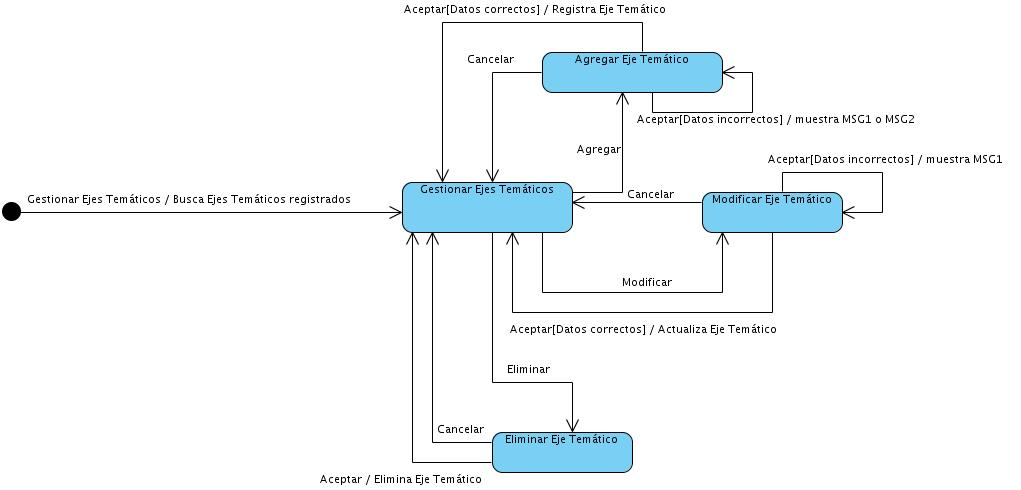
\includegraphics[width=0.8\textwidth]{images/CUG3/MapaNavegacion.jpg}
 		\caption{Mapa de navegacion para el CU G3 Gestion de Ejes Temáticos.}
		\label{fig:mapaNavegacionCUG3}
 	\end{figure}


\subsubsection{Objetivo}
Saber cuales son los ejes temáticos que están dadas de alta e interactuar con ellos. Vease Figura ~\ref{IUGestEjesTematicos} viene de Gestionar Catálogos.

\IUfig[0.6]{CUG3/GestionEjeTematico.PNG}{IUGestEjesTematicos}{Gestionar Ejes Temáticos.}

\subsubsection{Salidas}
Lista de Ejes Temáticos Registrados.

\subsubsection{Controles}
\begin{itemize}
 \item \IUbutton{Flecha derecha} Muestra los siguientes n ejes temáticos.
 \item \IUbutton{Flecha izquierda} Muestra los n ejes temáticos anteriores.
\end{itemize}

\newpage
\subsubsection{Comandos}
\begin{itemize}
 \item \IUbutton{
\includegraphics[scale=0.2]{images/icons/agregar.png}} Muestra la ventana \IUref{IUAgregarEjeTematico}{Agregar Eje Temático}.
 \item \IUbutton{
\includegraphics[scale=0.15]{images/icons/eliminar.png}}:Lleva a la pantalla \IUref{IUEliminarEjeTematico}{Eliminar Eje Temático}, en donde se podrá eliminar el eje temático de la fila donde se encuentra el botón. 
 \item \IUbutton{
\includegraphics[scale=0.15]{images/icons/editar.png}}: Permite modificar el eje temático que corresponde a la fila de este botón, lleva a la pantalla \IUref{IUModificarEjeTematico}{Modificar Eje Temático}.

\end{itemize}


